\documentclass[a4paper,14pt,russian]{extreport}

\hoffset 0pt
\voffset 0pt

\usepackage[
  a4paper, includehead, includefoot, mag=1000,
  headsep=0mm, headheight=0mm,
  left=25mm, right=15mm, top=20mm, bottom=20mm
]{geometry}

\usepackage[T2A]{fontenc}
\usepackage[utf8]{inputenc}
\usepackage[russian]{babel}

% \usepackage{cmap} % Улучшенный поиск русских слов в полученном pdf-файле
\usepackage[unicode, pdftex]{hyperref}
\usepackage{pdfpages}
\usepackage[nottoc]{tocbibind}

\usepackage[onehalfspacing]{setspace} %"умное" расстояние между строк - установить 1.5 интервала от нормального
\usepackage{cite}  %"умные" библиографические ссылки (сортировка и сжатие)
\usepackage{indentfirst} %делать отступ в начале параграфа
\usepackage{enumerate}  %создание и автоматическая нумерация списков
\usepackage{longtable} % Длинные таблицы
\usepackage{multirow,makecell,array} % Улучшенное форматирование таблиц
\usepackage{graphicx} \graphicspath{{images/}}
\usepackage{pdflscape} % Для включения альбомных страниц
\renewcommand{\rmdefault}{ftm} % Включаем Times New Roman
%%% Выравнивание и переносы %%%
\sloppy % Избавляемся от переполнений
\clubpenalty=10000 % Запрещаем разрыв страницы после первой строки абзаца
\widowpenalty=10000 % Запрещаем разрыв страницы после последней строки абзаца
\righthyphenmin=2 % Минимальное число символов при переносе - 2.

\usepackage{fancyvrb}

\usepackage{amssymb,amsmath,amsfonts,latexsym,mathtext} %расширенные наборы  математических символов

\usepackage{amsthm}
\theoremstyle{definition}
\newtheorem{theorem}{Теорема}
\newtheorem{proposition}[theorem]{Предложение}
\newtheorem{corollary}[theorem]{Следствие}
\newtheorem{lemma}[theorem]{Лемма}
\newtheorem{definition}[theorem]{Определение}
\newtheorem{example}[theorem]{Пример}
\newtheorem{remark}[theorem]{Замечание}

\usepackage[tableposition=top]{caption}
\DeclareCaptionLabelFormat{gostfigure}{Рисунок #2}
\DeclareCaptionLabelFormat{gosttable}{Таблица #2}
\DeclareCaptionLabelSeparator{gost}{~---~}
\captionsetup{labelsep=gost}
\captionsetup[figure]{labelformat=gostfigure}
\captionsetup[table]{labelformat=gosttable}

\usepackage{fancyhdr}

\pagestyle{fancyplain}
\renewcommand{\headrulewidth}{0pt}
\fancyhf{}
\rfoot{\fancyplain{}{\thepage}}

\makeatletter 
\renewcommand\chapter{\if@openright\cleardoublepage\else\clearpage\fi \thispagestyle{fancyplain}%
\global\@topnum\z@ \@afterindentfalse \secdef\@chapter\@schapter} 
\makeatother

\addtocontents{toc}{\protect\thispagestyle{fancyplain}}

\setcounter{page}{1}

\usepackage{titlesec}
\titleformat{\chapter}
	{\normalsize\bfseries}
	{\thechapter}
	{1em}{}
	
\titleformat{\section}
	{\normalsize\bfseries}
	{\thesection}
	{1em}{}
	
\titleformat{\subsection}
	{\normalsize\bfseries}
	{\thesubsection}
	{1em}{}

\titleformat{\paragraph}
	{\normalsize\bfseries}
	{\thesection}
	{1em}{}

	
\titlespacing*{\chapter}{0pt}{-30pt}{8pt}
\titlespacing*{\section}{\parindent}{*4}{*4}
\titlespacing*{\subsection}{\parindent}{*4}{*4}
\titlespacing*{\paragraph}{\parindent}{*4}{*4}

\addto\captionsrussian{%
  \renewcommand\contentsname{CОДЕРЖАНИЕ}
  \renewcommand\appendixname{ПРИЛОЖЕНИЕ}
  \renewcommand\bibname{СПИСОК ИСПОЛЬЗОВАННЫХ ИСТОЧНИКОВ}
}

\usepackage{enumitem}
\makeatletter
    \AddEnumerateCounter{\asbuk}{\@asbuk}{м)}
\makeatother
\setlist{nolistsep}
\renewcommand{\labelitemi}{-}
\renewcommand{\labelenumi}{\asbuk{enumi})}
\renewcommand{\labelenumii}{\arabic{enumii})}

\usepackage{tocloft}
\renewcommand{\cfttoctitlefont}{\hspace{0.38\textwidth} \bfseries\MakeUppercase}
\renewcommand{\cftbeforetoctitleskip}{-1em}
\renewcommand{\cftaftertoctitle}{\mbox{}\hfill \\ \mbox{}\hfill{\footnotesize Стр.}\vspace{-2.5em}}
\renewcommand{\cftchapfont}{\normalsize\bfseries}
\renewcommand{\cftsecfont}{\hspace{31pt}}
\renewcommand{\cftsubsecfont}{\hspace{11pt}}
\renewcommand{\cftbeforechapskip}{1em}
\renewcommand{\cftparskip}{-1mm}
\renewcommand{\cftdotsep}{1}
\renewcommand{\cftchapdotsep}{\cftdotsep}
\setcounter{tocdepth}{2} % задать глубину оглавления — до subsection включительно

\newcommand{\likechapterheading}[1]{
    \newpage
    \begin{center}
    \textbf{\MakeUppercase{#1}}
    \end{center}}

\newcommand{\abbreviations}{\likechapterheading{ОБОЗНАЧЕНИЯ И СОКРАЩЕНИЯ}\addcontentsline{toc}{chapter}{ОБОЗНАЧЕНИЯ И СОКРАЩЕНИЯ}}
\newcommand{\definitions}{\likechapterheading{ОПРЕДЕЛЕНИЯ}\addcontentsline{toc}{chapter}{ОПРЕДЕЛЕНИЯ}}
\newcommand{\abbrevdef}{\likechapterheading{ОПРЕДЕЛЕНИЯ, ОБОЗНАЧЕНИЯ И СОКРАЩЕНИЯ}\addcontentsline{toc}{chapter}{ОПРЕДЕЛЕНИЯ, ОБОЗНАЧЕНИЯ И СОКРАЩЕНИЯ}}
\newcommand{\intro}{\likechapterheading{ВВЕДЕНИЕ}\addcontentsline{toc}{chapter}{ВВЕДЕНИЕ}}
\newcommand{\conclusions}{\likechapterheading{ЗАКЛЮЧЕНИЕ}\addcontentsline{toc}{chapter}{ЗАКЛЮЧЕНИЕ}}

\makeatletter
  \renewcommand{\@biblabel}[1]{#1.}	% Заменяем библиографию с квадратных скобок на точку:
\makeatother

\newcommand{\biblio}{
  \bibliographystyle{ugost2008}	% Оформляем библиографию в соответствии с ГОСТ 7.0.5
  \nocite{*}
  \bibliography{biblio}
}

\newcommand{\appendxchapter}[1]{ 
    \clearpage
    \stepcounter{chapter}    
    \chapter*{\appendixname~\Asbuk{chapter}\;#1}
    \addcontentsline{toc}{chapter}{\appendixname~\Asbuk{chapter}\;#1}
}
 

%\graphicspath{{Graphs/}{e_0/}{e_0.25/}{e_0.5/}{medium_reorientation/}{large_reorientation/}%{variant_1/}{variant_2/}{variant_3/}}

\renewcommand{\rmdefault}{cmr} % Шрифт с засечками
\renewcommand{\sfdefault}{cmss} % Шрифт без засечек
\renewcommand{\ttdefault}{cmtt} % Моноширинный шрифт

\begin{document}

%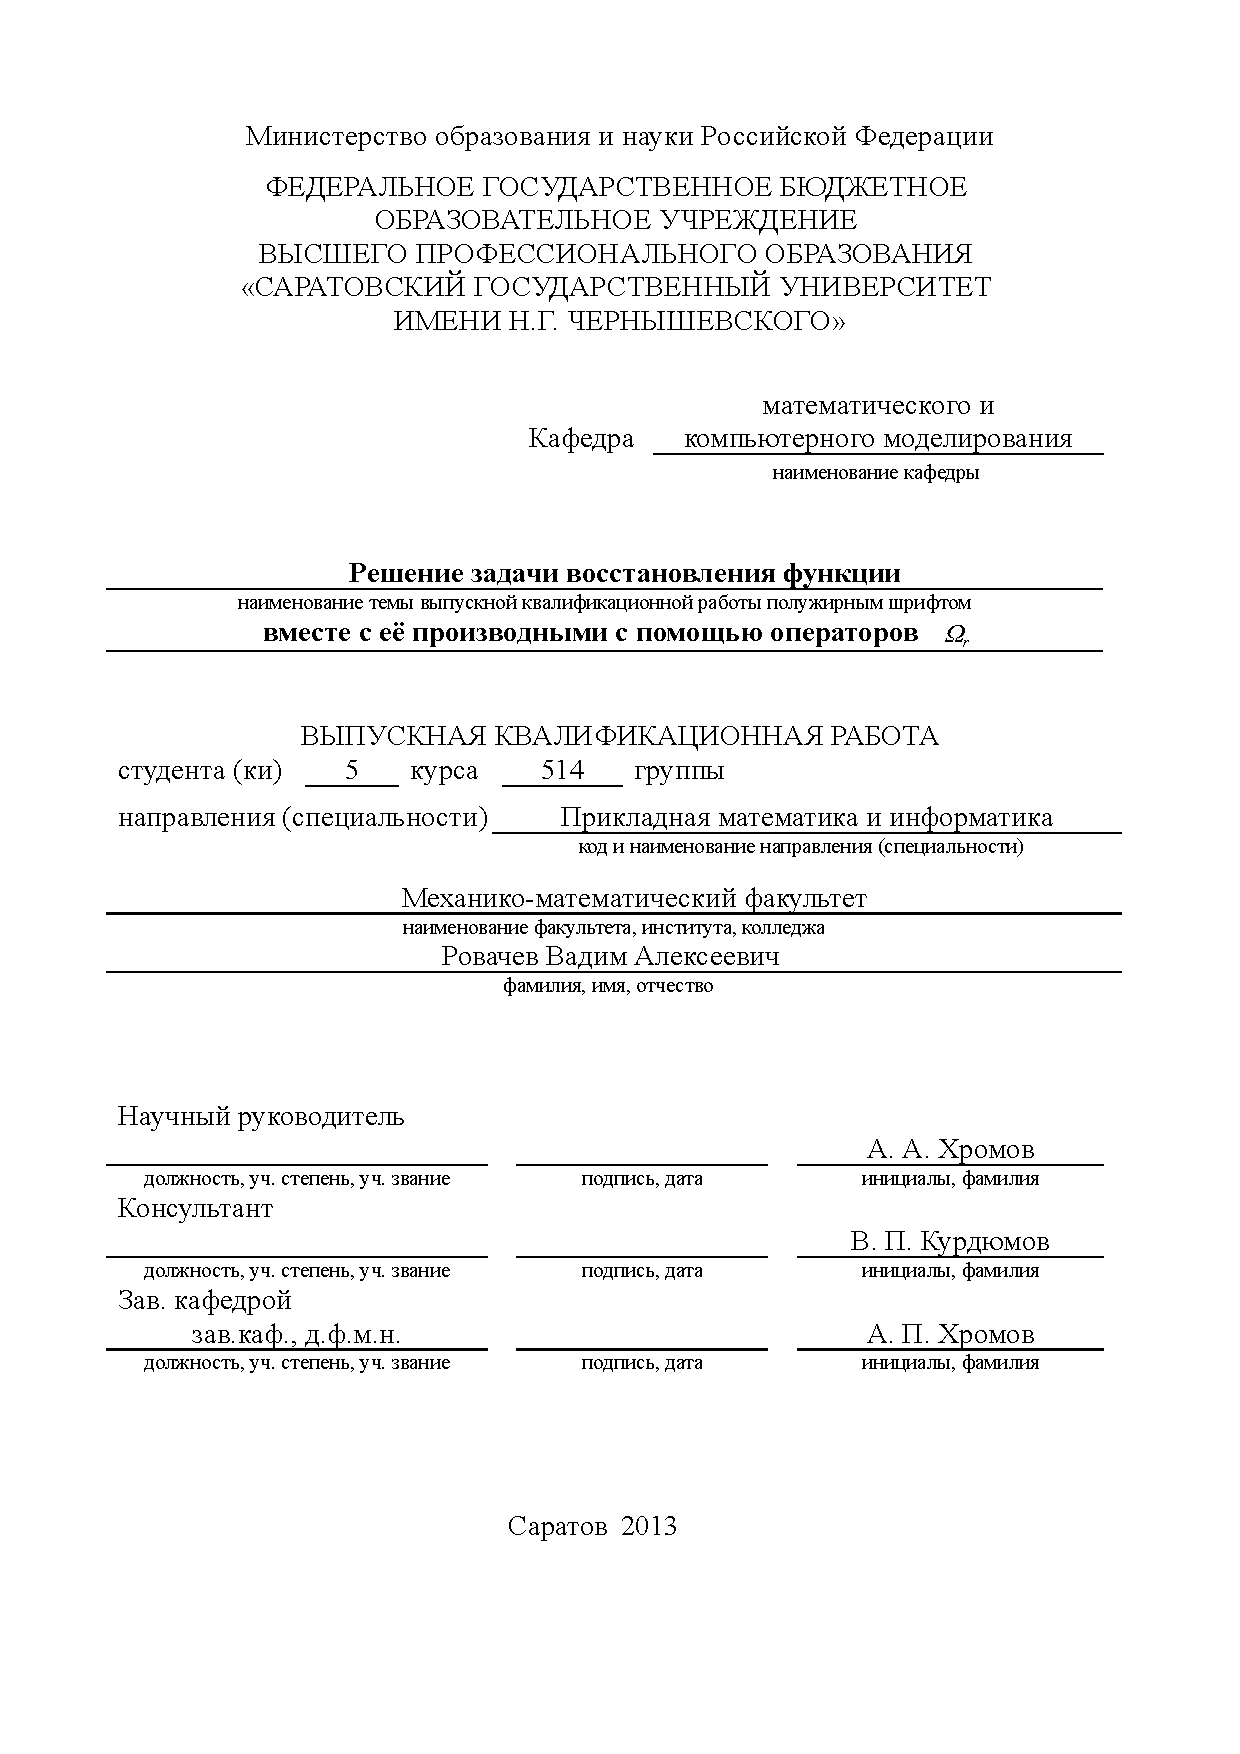
\includepdf[pages={1}]{titulDiplom.pdf}

\tableofcontents

\abbrevdef
\intro
\chapter{Приближающие свойства резольвенты оператора \\ $ L_1:y^{'}, y(0)=0 $ на отрезке $ [\varepsilon, 1] $.}
Рассмотрим простейший дифференциальный оператор первого порядка $ L_1:y^{'}, y(0)=0 $. Обозначим через $ R_\lambda(L_1) $ его резольвенту, т.е. оператор $ R_\lambda(L_1)=(L_1-\lambda E)^{-1} $, где $ E $ - единичный оператор, $ \lambda $ - спектральный параметр (числовой параметр,  вообще говоря, комплексный). Найдем формулу для резольвенты.

\section{Лемма 1.1}
\label{lemma1.1}

\textit{Для $ y(x) = R_\lambda(L_1)u$ имеет место формула:}

\begin{equation}
\begin{array}{c}

y(x) \equiv R_\lambda(L_1)u = \int\limits_0^x e^{\lambda(x-t)}u(t)dt.

\end{array}
\end{equation}

\textbf{Доказательство.} Пусть $ y = R_\lambda(L_1)u$. Тогда

\begin{equation}
\begin{array}{c}

y'- \lambda y = u,

\end{array}
\end{equation}

\begin{equation}
\begin{array}{c}

y(0)=0.

\end{array}
\end{equation}

По методу вариации произвольной постоянной общее решение уравнения (1.2) есть

\begin{equation}
\begin{array}{c}

y(x)=Ce^{\lambda x} + \int\limits_0^x e^{\lambda(x-t)}u(t)dt,

\end{array}
\end{equation}

Где $ C $ - произвольная постоянная. Находим эту постоянную из условия (1.3). Получаем $ C = 0 $. Отсюда приходим к формуле (1.1).
	
Положим в (1.1) $ \lambda \ -r $, где $ r > 0 $, и рассмотрим операторы $ rR_{-r}(L_1)$. Очевидно, эти операторы имеют вид:

\begin{equation}
\begin{array}{c}

rR_{-r}(L_1)u = r \int\limits_0^x e^{-r(x-t)}u(t)dt

\end{array}
\end{equation}

Выясним приближающие свойства операторов (1.5) при $ r \rightarrow \infty$.

\section{Лемма 1.2}
\label{lemma1.2}

\textit{Для любой функции $ u(x) \in C[0,1] $ имеет место сходимость:}

\begin{equation}
\begin{array}{c}

\Vert rR_{-r}(L_1)u-u \Vert _{C[\varepsilon ,1]} \rightarrow 0 $ \textit{при} $ r \rightarrow \infty,

\end{array}
\end{equation}

\textit{ $ \varepsilon $ - произвольное малое положительное число.}

\textbf{Доказательство.} Пусть сначала $ u(x) \in C^1[0,1] $. Тогда

\begin{equation}
\begin{array}{c}
\nonumber

\int\limits_0^x e^{-r(x-t)}u(t)dt = \frac{1}{r}\bigl\vert_0^x e^{-r(x-t)}u(t) - \frac{1}{r}\int\limits_0^x e^{-r(x-t)}u'(t)dt = \\
= \frac{1}{r} \bigl[u(x)-e^{-rx}u(0)-\int\limits_0^x e^{-r(x-t)}u'(t)dt\bigl].

\end{array}
\end{equation}

Отсюда получаем

\begin{equation}
\begin{array}{c}
\nonumber

rR_{-r}(L_1)u = u(x) - e^{-rx}u(0) - \frac{1}{r} (rR_{-r}(L_1)u').

\end{array}
\end{equation}

Тогда

\begin{equation}
\begin{array}{c}
\nonumber

rR_{-r}(L_1)u - u = u(x) - e^{-rx}u(0) - \int\limits_0^x e^{-r(x-t)}u'(t)dt.

\end{array}
\end{equation}

Далее,

\begin{equation}
\begin{array}{c}
\nonumber

\bigl| \int\limits_0^x e^{-r(x-t)}u'(t)dt \bigr| \leq \Vert u' \Vert_{C[0,1]} \int\limits_0^x e^{-r(x-t)}dt = \\
= \frac{1}{r} \Vert u' \Vert_{C[0,1]}.
(1 - e^{-rx}) 
\end{array}
\end{equation}

Тогда

\begin{equation}
\begin{array}{c}

\bigl| rR_{-r}(L_1)u - u \bigr| \leq e^{-rx} \bigl| u(0) \bigr| + \dfrac{1}{r} (1-e^{-rx})\Vert u' \Vert_{C[0,1]}.

\end{array}
\end{equation}

В силу того, что первое слагаемое в правой части последней оценки при $ x = 0 $ является константой, не зависящей от $ r $, то на всем отрезке $ [0,1] $ сходимости функций $ rR_{-r}(L_1)u $ к $ u(x) $ при $ r \rightarrow \infty $ мы отсюда не получим. Но если мы рассмотрим отрезок $ [\varepsilon, 1] $, где $ \varepsilon > 0 $ - любое фиксированное как угодно малое число, то тогда $ \Vert e^{-rx}_{C[\varepsilon,1]} = e^{-r\varepsilon} \rightarrow 0 \Vert $ при $ r \rightarrow \infty $. Отсюда следует утверждение леммы для $ u \in C^1[0,1] $.

Пусть теперь $ u(x) \in C[0,1] $. Покажем, что нормы операторов $ eR_{-r}(L_1) $, рассматриваемых как операторы из $  C[0,1] $ в $ C[\varepsilon,1] $, ограничены константой, не зависящей от $ r $.

Действительно, имеем:

\begin{equation}
\begin{array}{c}

\Vert rR_{-r}(L_1)u \Vert_{C[\varepsilon,1]} \leq \Vert rR_{-r}(L_1)u \Vert_{C[0,1]} = \\
= \bigl\Vert r\int\limits_0^x e^{-r(x-t)}u(t)dt\bigr\Vert_{C[0,1]} \leq \Vert u\Vert_{C[0,1]}\Vert 1 - e^{-rx}\Vert_{C[0,1]} \leq \Vert u \Vert_{C[0,1]}.

\end{array}
\end{equation}

Далее, множество функций $ u \in C^1[0,1] $ является всюду плотным в пространстве $ C[0,1] $. (Это следует из теоремы Вейерштрасса об аппроксимации непрерывной функции полиномами). Поэтому по теореме Банаха- Штейнгауза из ограниченности норм операторов $ rR_{-r}(L_1) $ отсюда следует сходимость (1.6) для любой $ u \in C[0,1] $.

Лемма доказана.

Покажем теперь, что приближающие свойства операторов $ rR_{-r}(L_1) $ сохраняются и в пространствах гладких функций, т.е. в пространствах $ C^l[0,1] $.

Пусть сначала $ u \in C^{l-1}[0,1] $. Рассмотрим операторы $ D^kR_{-r}(L_1) \equiv (R_{-r}(L_1)u)_x^{(k)} k = 1,...,l, D^1 \equiv D (Du = u')$.

\section{Лемма 1.3}
\label{lemma1.3}

\textit{Операторы $ D^kR_{-r}(L_1) $ имеют вид:}

\begin{equation}
\begin{array}{c}

D^kR_{-r}(L_1)u = u^{(k-1)}(x) - ru^{(k-2)}(x) + r^2u^{(k-3)}(x) - ... + \\
+ (-1)^{k-1}r^{k-1}u(x) + (-1)^kr^k\int\limits_0^x e^{-r(x-t)}u(t)dt, k = 1,...,l.

\end{array}
\end{equation}

\textbf{Доказательство.} Для $ k = 1 $ имеем:

\begin{equation}
\begin{array}{c}
\nonumber

DR_{-r}(L_1)u = (DR_{-r}(L_1)u)_x' = \bigl( \int\limits_0^x e^{-r(x-t)}u(t)dt \bigr)_x' = \\
= u(x) -r\int\limits_0^x e^{-r(x-t)}u(t)dt.

\end{array}
\end{equation}

Применяем метод математической индукции. Пусть (1.9) выполняется для $ k = m - 1 $, т.е.

\begin{equation}
\begin{array}{c}
\nonumber

D^{m-1}R_{-r}(L_1)u = u^{(m-2)}(x) - ru^{(m-3)}(x) + ... + \\
+ (-1)^{m-2}r^{m-2}u(x) + (-1)^{m-1}r^{m-1}\int\limits_0^x e^{-r(x-t)}u(t)dt.

\end{array}
\end{equation}

Тогда для $ k = m $ получим:

\begin{equation}
\begin{array}{c}
\nonumber

D^{m}R_{-r}(L_1)u = D(D^{m-1}R_{-r}(L_1)u) = u^{(m-1)}(x) - ru^{(m-2)}(x) + ... + \\
+ (-1)^{m-2}r^{m-2}u'(x) + (-1)^{m-1}r^{m-1}u(x) + (-1)^mr^m\int\limits_0^x e^{-r(x-t)}u(t)dt.

\end{array}
\end{equation}

Лемма доказана.

\section{Лемма 1.4}
\label{lemma1.4}

\textit{Если $ u(x) \in C^l[0,1] $, то имеет место сходимость:}

\begin{equation}
\begin{array}{c}

\Vert rD^k R_{-r}(L_1)u -u^{(k)}(x) \Vert_{C[\varepsilon ,1} \rightarrow 0 $ \textit{при} $ r \rightarrow \infty, k = 1,...,l.

\end{array}
\end{equation}

\textit{ $ \varepsilon $ - произвольное малое положительное число.}

\textbf{Доказательство.} Пусть $ k = 1 $. По лемме 1.3 имеем:

\begin{equation}
\begin{array}{c}

DR_{-r}(L_1)u = u(x) - r\int\limits_0^x e^{-r(x-t)}u(t)dt.

\end{array}
\end{equation}

Далее,

\begin{equation}
\begin{array}{c}

\int\limits_0^x e^{-r(x-t)}u(t)dt = e^{-rx}\int\limits_0^x e^{rt}u(t)dt = \\
= e^{-rx} \big\vert_0^x \frac{1}{r} e^{rt}u(t) - \frac{1}{r}\int\limits_0^x e^{-r(x-t)}u'(t)dt = \\
= \frac{1}{r}u(x) - \frac{1}{r} e^{-rx}u(0) - \frac{1}{r}\int\limits_0^x e^{-r(x-t)}u'(t)dt

\end{array}
\end{equation}

Подставляя (1.12) в (1.11), получим:

\begin{equation}
\begin{array}{c}
\nonumber

DR_{-r}(L_1)u = e^{-rx}u(0) + \int\limits_0^x e^{-r(x-t)}u'(t)dt

\end{array}
\end{equation}

или

\begin{equation}
\begin{array}{c}

DR_{-r}(L_1)u = R_{-r}(L_1)u' + e^{-rx}u(0).

\end{array}
\end{equation}

Получим аналогичное (1.13) выражение для $ D^kR_{-r}(L_1) $ при $ k > 1 $. 

В силу (1.13) имеем:

\begin{equation}
\begin{array}{c}
\nonumber

D^2R_{-r}(L_1)u = D(DR_{-r}(L_1)u) = D[R_{-r}(L_1)u' + e^{-rx}u(0)] = \\
= DR_{-r}(L_1)u' - re^{-rx}u(0).

\end{array}
\end{equation}

Опять применяем (1.13), заменив $ u $ на $ u' $.

Получаем:

\begin{equation}
\begin{array}{c}
\nonumber

D^2R_{-r}(L_1)u = R_{-r}(L_1)u'' + e^{-rx}u'(0) - re^{-rx}u(0).

\end{array}
\end{equation}

Покажем, что в общем случае для любого $ k $ справедлива формула:

\begin{equation}
\begin{array}{c}

D^kR_{-r}(L_1)u = R_{-r}(L_1)u^{(k)} + e^{-rx}u^{(k-1)}(0) -er^{-rx}u^{(k-2)}(0) + ... + \\
+ (-1)^{k-1}r^{k-1}e^{-rx}u(0).

\end{array}
\end{equation}

Мы показали, что (1.14) выполняется для $ k = 1,2 $. Пусть это соотношение выполняется для $ k = m - 1 $, т.е.

\begin{equation}
\begin{array}{c}
\nonumber

D^{m-1}R_{-r}(L_1)u = R_{-r}(L_1)u^{(m-1)} + e^{-rx}u^{(m-2)}(0) - re^{-rx}u^{(m-3)}(0) + ... + \\
+ (-1)^{m-2}r^{m-2}e^{-rx}u(0).

\end{array}
\end{equation}

Тогда

\begin{equation}
\begin{array}{c}
\nonumber

D^mR_{-r}(L_1)u = D(D^{m-1}R_{-r}(L_1)u) = DR_{-r}(L_1)u^{(m-1)} + \\
+ D\bigl[e^{-rx}u^{(m-2)}(0) - re^{-rx}u^{(m-3)}(0) + ... + (-1)^{m-2}r^{m-2}e^{-rx}u(0)\bigr].

\end{array}
\end{equation}

Используя (1.13) с заменой $ u(x) $ на $ u^{(m-1)}(x) $, придём к выражению:

\begin{equation}
\begin{array}{c}
\nonumber

D^mR_{-r}(L_1)u = R_{-r}(L_1)u^{(m)} + e^{-rx}u^{(m-1)}(0) - re^{-rx}u^{(m-2)}(0) + \\
+ r^2e^{-rx}u^{(m-3)}(0) + ... + (-1)^{m-1}r^{m-1}e^{-rx}u(0).

\end{array}
\end{equation}

Из формулы (1.14) получаем оценку:

\begin{equation}
\begin{array}{c}
\nonumber

\bigl\Vert rD^kR_{-r}(L_1)u - u^{(k)}\bigr\Vert_{C[\varepsilon ,1]} \leq \bigl\Vert rR_{-r}(L_1)u^{(k)} - u^{(k)}\bigr\Vert_{C[\varepsilon ,1]} + e^{-r\varepsilon}\sum\limits_{j=0}^{k-1} r^j\vert u^{(k-j-1)}(0)\vert,

\end{array}
\end{equation}

И тогда соотношение (1.10) вытекает из леммы 1.2.

\textbf{Замечание}. Если в лемме 1.2 $ u(0) = 0 $, то сходимость (1.6) будет выполняться при $ \varepsilon = 0$, т.е. на всем отрезке $ [0,1] $. Если в лемме 1.4 $ u^{(m)}(0) = 0, m = 0,1,...,k $, , то сходимость 1.10 будет выполняться также при $ \varepsilon = 0 $.

В дальнейшем нам потребуются свойства не только самих операторов $ rR_{-r}(L_1) $, но и их степеней – операторов $ (rR_{-r}(L_1))^k $.

\section{Лемма 1.5}
\label{lemma1.5}

\textit{Операторы $ (rR_{-r}(L_1))^k $ имеют вид:}

\begin{equation}
\begin{array}{c}

(rR_{-r}(L_1))^ku = r^k\int\limits_0^x \dfrac{(x-t)^{k-1}}{(k-1)!}e^{-r(x-t)}u(t)dt.

\end{array}
\end{equation}

\textbf{Доказательство.} Обозначим для краткости $ rR_{-r}(L_1) = \Omega_{1r} $. Тогда для $ k = 2 $ имеем:

\begin{equation}
\begin{array}{c}
\nonumber

\Omega_{1r}^2u = r^2\int\limits_0^x e^{-r(x-t)} \int\limits_0^t e^{-r(x-t)} u(\tau)d\tau dt = \\
= r^2e^{-rx}\int\limits_0^x\int\limits_0^t e^{r\tau}u(\tau)d\tau dt = r^2e^{-rx}\int\limits_0^x\int\limits_\tau^x dte^{r\tau}u(\tau)d\tau = \\
= r^2e^{-rx}\int\limits_0^x (x-\tau)e^{r\tau}u(\tau)d\tau = r^2\int\limits_0^x (x-\tau)e^{-r(x-t)}u(\tau)d\tau .

\end{array}
\end{equation}

Заменим обозначение $ \tau $ на $ t $, получим (1.15) при $ k = 2 $. 

Пусть для $ k = m - 1 $ выполняется формула (1.15), т.е.

\begin{equation}
\begin{array}{c}
\nonumber

\Omega_{1r}^{m-1}u = r^{m-1}\int\limits_0^x\dfrac{(x-t)^{m-2}}{(m-2)!}e^{-r(x-t)}u(t)dt.

\end{array}
\end{equation}

Тогда

\begin{equation}
\begin{array}{c}
\nonumber

\Omega_{1r}^mu = \Omega_{1r}(\Omega_{1r}^{m-1}u) = r^m\int\limits_0^x e^{-r(x-t)} \int\limits_0^t\dfrac{(t-\tau)^{m-2}}{(m-2)!}e^{-r(t-\tau)}u(\tau)d\tau dt = \\
= r^me^{-rx}\int\limits_0^x\int\limits_0^t\dfrac{(t-\tau)^{m-2}}{(m-2)!}e^{r\tau}u(\tau)d\tau dt = \\
= r^me^{-rx}\int\limits_0^x\int\limits_\tau^x\dfrac{(t-\tau)^{m-2}}{(m-2)!}dte^{r\tau}u(\tau)d\tau = \\
= r^m\int\limits_0^x\dfrac{(x-\tau)^{m-1}}{(m-1)!}e^{-r(x-t)}u(\tau)d\tau,

\end{array}
\end{equation}

что и требовалось доказать.

\section{Лемма 1.6}
\label{lemma1.6}

\textit{Если $ u \in C^1[0,1] $, то операторы $ \Omega_{1r}^k $ имеют представление:}

\begin{equation}
\begin{array}{c}

\Omega_{1r}^ku = -\dfrac{r^{k-1}x^{k-1}e^{-rx}}{(k-1)!}u(0) + \Omega_{1r}^{k-1}u - \dfrac{1}{r}\Omega_{1r}^ku',

\end{array}
\end{equation}

\textit{где $ k \geq 2 $.}

\textbf{Доказательство.} Пусть $ k = 2 $.  Тогда из (1.15) мы получаем:

\begin{equation}
\begin{array}{c}
\nonumber

\Omega_{1r}^2u = r^2\int\limits_0^x (x-t)e^{-r(x-t)}u(t)dt.

\end{array}
\end{equation}
Интегрируем по частям:
\begin{equation}
\begin{array}{c}
\nonumber

\Omega_{1r}^2u = r^2\bigl\lbrace \frac{1}{r} \big\vert_0^x e^{-r(x-t)}(x-t)u(t) - \frac{1}{r} \int\limits_0^x e^{-r(x-t)}[-u(t) + (x - t)u'(t)]dt \bigr\rbrace = \\
= r \bigl[ -xe^{-rx}u(0) + \int\limits_0^x e^{-r(x-t)}u(t)dt - \int\limits_0^x e^{-r(x-t)}(x-t)u'(t)dt \bigr] = \\
= -rxe^{-rx}u(0) + \Omega_{1r}u - \dfrac{1}{r}\Omega_{1r}^2u'.

\end{array}
\end{equation}

Предположим, что (1.16) выполняется для $ k = m - 1, m > 2 $. Тогда

\begin{equation}
\begin{array}{c}
\nonumber

\Omega_{1r}^{m-1}u = -\dfrac{r^{m-2}x^{m-2}e^{-rx}}{(m-2)!}u(0) + \Omega_{1r}^{m-2}u - \dfrac{1}{r}\Omega_{1r}^{m-1}u.

\end{array}
\end{equation}

Отсюда

\begin{equation}
\begin{array}{c}
\nonumber

\Omega_{1r}^mu = r\int\limits_0^x e^{r(x-t)}\bigl[ -\dfrac{r^{m-2}t^{m-2}e^{-rt}}{(m-2)!}u(0) \bigr]dt + \Omega_{1r}(\Omega_{1r}^{m-2}u) - \dfrac{1}{r}\Omega_{1r}(\Omega_{1r}^{m-1}u') = -\dfrac{r^{m-1}x^{m-1}e^{-rx}}{(m-1)!}u(0) + \Omega_{1r}^{m-1}u - \dfrac{1}{r}\Omega_{1r}^mu',

\end{array}
\end{equation}

что и требовалось доказать.

\section{Лемма 1.7}
\label{lemma1.7}

\textit{Для $ u(x) \in C[0,1] $ справедливы соотношения:}

\begin{equation}
\begin{array}{c}

\Vert \Omega_{1r}^ku - u \Vert_{C[\varepsilon ,1]} \rightarrow 0 $ \textit{при} $ r \rightarrow \infty , k = 1,2,...

\end{array}
\end{equation}

\textbf{Доказательство.} Для $ k = 1 $ соотношение (1.17) доказано в Лемме 1.2.
Пусть $ k \geq 2 $, а $ u(x) \in C^k[0,1] $ обозначим $ \varphi_l(r,x) = - \dfrac{r^lx^le^{-rx}}{l!} $.
Из (1.16) имеем:

\begin{equation}
\begin{array}{c}
\nonumber

\Vert \Omega_{1r}^ku - u \Vert_{C[\varepsilon ,1]} \leq \Vert \varphi_{k-1}(r,x)u(0) \Vert_{C[\varepsilon, 1]} + \Vert \Omega_{1r}^{k-1}u - u \Vert_{C[\varepsilon ,1]} + \Vert \dfrac{1}{r}\Omega_{1r}^ku' \Vert_{C[\varepsilon, 1]} \leq \Vert \varphi_{k-1}(r,x)u(0) \Vert_{C[\varepsilon, 1]} + \Vert \varphi_{k-2}(r,x)u(0) \Vert_{C[\varepsilon, 1]} + ... + \Vert \varphi_1(r,x)u(0) \Vert_{C[\varepsilon, 1]} + \Vert \Omega_{1r}u - u \Vert_{C[\varepsilon ,1]} + \Vert \dfrac{1}{r}\Omega_{1r}^2u' \Vert_{C[\varepsilon, 1]} + \Vert \dfrac{1}{r}\Omega_{1r}^3u' \Vert_{C[\varepsilon, 1]} + ... + \Vert \dfrac{1}{r}\Omega_{1r}^ku' \Vert_{C[\varepsilon, 1]}.

\end{array}
\end{equation}

Далее, поскольку $ \varphi_l(r,x) \leq r^le^{-r\varepsilon} $ на отрезке $ [\varepsilon ,1] $, то сумма слагаемых, содержащих функции $ \varphi_l(r,x), l = 1,...,k-1  $, имеет оценку $ O(r^{k-1}e^{-r\varepsilon}\Vert u \Vert_{C[0,1]}) $.

По лемме 1.2 $ \Vert \Omega_{1r}u - u \Vert_{C[\varepsilon ,1]} \rightarrow 0 $ при $ r \rightarrow \infty $ для любой $ u(x) \in C[0,1] $. 

Осталось показать, что слагаемые, содержащие $ u'(x) $, могут быть как угодно малыми при $ r \rightarrow \infty $, если $ u(x) \in C^k[0,1] $, т.е., что $ \bigl\Vert \dfrac{1}{r}\Omega_{1r}^lu' \bigr\Vert_{C[\varepsilon ,1]} \rightarrow 0$ при $ r \rightarrow \infty $ для $ l = 2,...,k $.

Пусть $ l = 2 $. Тогда из (16) с заменой $ u $ на $ u' $ получим:

\begin{equation}
\begin{array}{c}
\nonumber

\dfrac{1}{r}\Omega_{1r}^2u' = -xe^{-rx}u'(0) + \dfrac{1}{r}\Omega_{1r}u' - \dfrac{1}{r^2}\Omega_{1r}^2u''.

\end{array}
\end{equation}

Но $ \dfrac{1}{r}\Omega_{1r}u' $ и $ \dfrac{1}{r^2}\Omega_{1r}^2u'' $ есть $ O(\dfrac{1}{r}) $. Действительно,

\begin{equation}
\begin{array}{c}
\nonumber

\dfrac{1}{r}\vert\Omega_{1r}u'\vert = \bigl\vert \int\limits_0^x e^{-r(x-t)}u'(t)dt \bigr\vert \leq \Vert u' \Vert_{C[0,1]} \int\limits_0^x e^{-r(x-t)}dt = \dfrac{1}{r}(1 - e^{-rx})\Vert u' \Vert_{C[0,1]} \leq \dfrac{1}{r} \Vert u' \Vert_{C[0,1]}.

\end{array}
\end{equation}

И точно так же

\begin{equation}
\begin{array}{c}
\nonumber

\dfrac{1}{r^2} \vert \Omega_{1r}^2u'' \vert = \bigl| \int\limits_0^x e^{-r(x-t)}(x-t)u''(t)dt \bigr| \leq \dfrac{1}{r} \Vert u'' \Vert_{C[0,1]}.

\end{array}
\end{equation}

Для произвольного $ l $ из (1.16) получаем:

\begin{equation}
\begin{array}{c}

\dfrac{1}{r} \Omega_{1r}^lu' = \dfrac{1}{r} \varphi_{l-1}(r,x)u'(0) + \dfrac{1}{r}\Omega_{1r}^{l-1}u' - \dfrac{1}{r^2} \Omega_{1r}^lu''.

\end{array}
\end{equation}

Из (1.15) имеем:

\begin{equation}
\begin{array}{c}

\dfrac{1}{r}\Omega_{1r}^{l-1}u' = r^{l-2}\int\limits_0^x e^{-r(x-t)}\dfrac{(x-t)^{l-2}}{(l-2)!}u'(t)dt,

\end{array}
\end{equation}

\begin{equation}
\begin{array}{c}

\dfrac{1}{r^2} \Omega_{1r}^lu'' = r^{l-2}\int\limits_0^x e^{-r(x-t)}\dfrac{(x-t)^{l-1}}{(l-1)!}u''(t)dt.

\end{array}
\end{equation}



\end{document}